% !TEX root = ../chrysalis-report.tex
%
\section{Ethereum overhaul}
\label{sec:impr:eth}

In this section we will discuss improvements regarding the smart contract structure of the project. Smart contracts are used for the deployment and execution of process instances within the system. They contain structures and methods for creation and handling of tasks and control flow decisions. For each process instance one new instance of the BasicEnzian smart contract is deployed.

\subsection{Problem statement}
\label{sec:impr:eth:problem}

In its initial state, the project kept all of its on-chain functionality in one single smart contract. There was no separation of concerns, a lot of the universal, non instance-specific functionality was left in, which lead to not only poor scalability and reusability of the smart contract code in the future, but also to significant performance costs, which, on the ethereum network, are measured in a unit called "gas". Gas consumption defines how much computational power the network needs to execute a certain operation, which then determines how much currency should be transferred from the account of a node requesting to execute this operation, to the account of the owner of the node executing it. So in case of Ethereum, performance costs literally translate to money spent, that is why the main goal of the optimization was to minimize them. The listing below provides an example of code redundancy within the smart contract functionality. It contains a part of the task execution function, and as can be seen, mostly consists of parts which do not have to be in the contract and could be delegated to external components.

\lstinputlisting[style=java,caption=Task execution before the optimization]{progs/executeTask-before.txt} 

\subsection{Solution}
\label{sec:impr:eth:solution}

To achieve this, we had to optimize the most expensive operation in our system - smart contract deployment, since it happens for every new process instance in the system. Also the issue of reusability of components becomes more crucial, because as the project will become progressively more complex in the future, the on-chain functionality will do so as well, so we have to split the smart contract code into elementary parts, which would allow to implement new features by adding and deploying new modules, using existing ones, instead of rewriting and redeploying everything, which would also decrease performance costs during future development.

As an implementation model for this task clean architecture was chosen, since this model is designed to increase reusability of application components and overall scalability of the application. The main principle of this model is that all the modules are diveded into three layers - domain layer, application layer and presentation layer. Domain layer defines structures and entities used in the application, basic objects carrying its state. Application layer, or middle layer, contains business logic of the application, the modules responsible for its behaviour, dealing with the object from the domain layer. Presentation layer provides entry points for external systems and users, that call functions and methods of the middle layer. The main requirement is that modules can only interact either with the modules from the same layer or the inner layer modules.

\subsection{Implementation}
\label{sec:impr:eth:implementation}

On the domain model layer, the libraries containing structs defining the objects of a process model along with the process state were implemented. These libraries were TaskEntities, DecisionEntities and ProcessEntities.\newline
TaskEntities library define the structure of a process task, which contains information on Tasks name and id within the process instance, its completion state, as well as the set of requirements, that have to be fulfilled for this task to be up for execution. It also contains a reference to a Decision object, which is described in the DecisionEntities library.

DecisionEntities library defines structures and enumerators needed for evaluating control flow requirements in the gateways of a process model. The decision structure utself contains information on the gateway type, variables compared as well as the comparison operator for those variables. The enumerators containing gateway types and operators are also defined in this library.\newline
ProcessEntities library defines the structure containing information on the process structure and state. It contains the process' tasks, its integer variables and string variables.

On the application layer there are two libraries: TaskLibrary and DecisionLibrary. TaskLibrary implements methods creating tasks on the process initialization, as well as methods handling execution of tasks including evaluation of task requirements. To evaluate gateway conditions it calls the DecisionLibrary, which implements appropriate functionality.\newline
The presentation layer consists of the BasicEnzian smart contract, which provides entry points for the EnzianYellow library to interact with, as well as keeps the state of the process instance and its event log. 

\begin{figure}[h]
	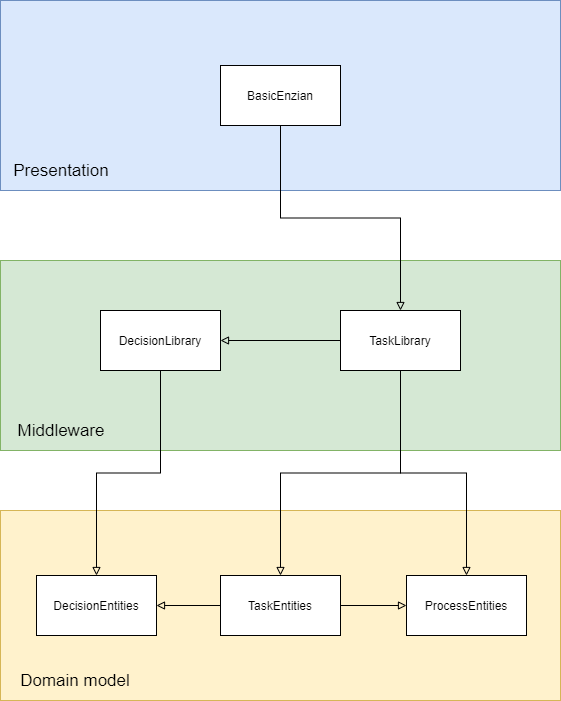
\includegraphics[width=\textwidth]{gfx/eth-contracts}
	\caption{Structure of the ethereum smart contracts}
	\label{fig:impr:eth:contracts}
\end{figure}

\subsection{Result}
\label{sec:impr:eth:result}

As an outcome of the smart contract overhaul, the structure of the smart contract code became more scalable and flexible, it was divided into small modules which can be reused in the new contracts developed further down the line.
Other than that, the cost of process instance deployment was lowered from ~4300000 gas to ~3600000 gas, and overall the code became much cleaner, which could be seen in the following listing, which showcases the same function handling task execution. After the refactoring most of the method's logic is incapsulated in the TaskLibrary, which is called, and then the results from the library function are used to update process state.

\lstinputlisting[style=java,caption=Task execution after the optimization]{progs/executeTask-after.txt} 

